% Section content template for individual Educative lessons
% This file contains the actual content for a specific section
% Generated from Educative API section content

% Section: Detailed Design of Uber
% Section ID: 6683135341494272
% Section Slug: detailed-design-of-uber
% Generated: 2025-12-07T23:31:42.930722

Let's look at the detailed design of our Uber system and learn how the various components work together to offer a functioning service:

\begin{figure}[htbp]
 \centering
 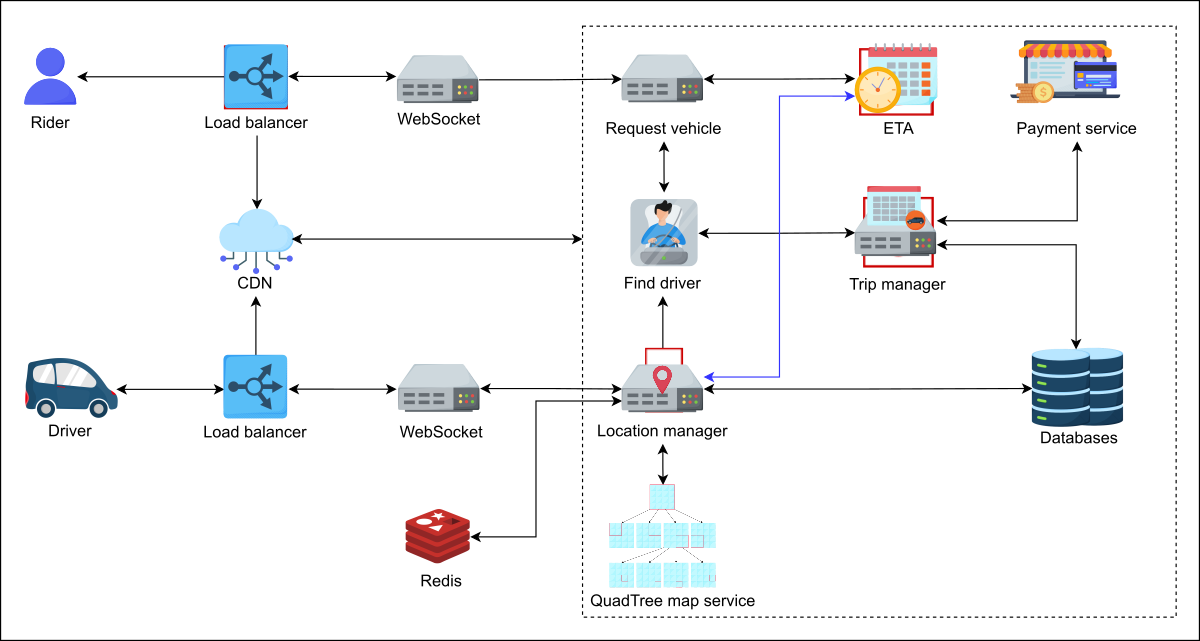
\includegraphics[width=0.5\textwidth]{Images/chapter_30/section_6683135341494272/5316575081398272.png}
 \caption{The detailed design of Uber}
\end{figure}

\subsection{Components}\label{p-lQpa8Ht_Sr8cIGox7rq}
\\
Let's discuss the components of our Uber system design in detail.

\subsubsection{Location manager}\label{txBsc9-jwu3vYmYFAOL8b}
\\
The riders and drivers are connected to the \textbf{location manager} service. This service shows the nearby drivers to the riders when they open the application. This service also receives location updates from the drivers every four seconds. The location of drivers is then communicated to the QuadTree map service to determine which segment the driver belongs to on a map. The location manager saves the last location of all drivers in a database and saves the route followed by the drivers on a trip.

\subsubsection{QuadTree map service}\label{T7Mry4tG8vRwlfA_c4EM1}
\\
The \textbf{QuadTree map service} updates the location of the drivers. The main problem is how we deal with finding nearby drivers efficiently.
\\
We'll modify the solution discussed in the \href{https://www.educative.io/courses/grokking-the-system-design-interview/system-design-yelp}{Yelp} chapter according to our requirements. We used QuadTrees(A QuadTree is a tree data structure in which each internal node has exactly four children. Quad Trees are the two-dimensional analog of octrees and are most often used to partition a two-dimensional space by recursively subdividing it into four quadrants or regions. The data associated with a leaf cell varies by application, but the leaf cell represents a ``unit of interesting spatial information''. Source
: Wikipedia) on Yelp to find the location. QuadTrees help to divide the map into segments. If the number of drivers exceeds a certain limit, for example, 500, then we split that segment into four more child nodes and divide the drivers among them.
\\
Each leaf node in QuadTrees contains segments that can't be divided further. We can use the same QuadTrees for finding the drivers. The most significant difference we have now is that our QuadTree wasn't designed with regular upgrades in consideration. So , we have the following issues with our dynamic segment solution.
\\
We must update our data structures to point out that all active drivers update their location every four seconds. It takes a longer amount of time to modify the QuadTree whenever a driver's position changes. To identify the driver's new location, we must first find a proper grid depending on the driver's previous position. If the new location doesn't match the current grid, we should remove the driver from the current grid and shift it to the correct grid. We have to repartition the new grid if it exceeds the driver limit, which is the number of drivers for each region that we set initially. Furthermore , our platform must tell both the driver and the rider, of the car's current location while the ride is in progress.
\\
To overcome the above problem, we can use a hash table to store the latest position of the drivers and update our QuadTree occasionally, say after 10--15 seconds. We can update the driver's location in the QuadTree around every 15 seconds instead of four seconds, and we use a hash table that updates every four seconds and reflects the drivers' latest location. By doing this, we use fewer resources and time.

\begin{figure}[htbp]
 \centering
 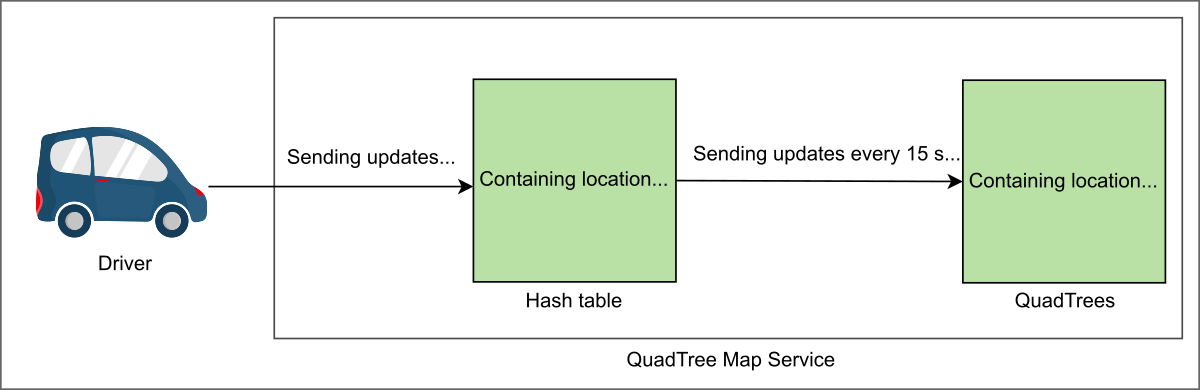
\includegraphics[width=0.5\textwidth]{Images/chapter_30/section_6683135341494272/5553535295160320.png}
 \caption{Updating driver's location}
\end{figure}

\subsubsection{Request vehicle}\label{O3FuZzj1cZQCATzc6qBn0}
\\
The rider contacts the \textbf{request vehicle} service to request a ride. The rider adds the drop-off location here. The request vehicle service then communicates with the find driver service to book a vehicle and get the details of the vehicle using the location manager service.

\subsubsection{Find driver}\label{LE6nVbkCpklzhyhbbLHT1}
\\
The \textbf{find driver} service finds the driver who can complete the trip. It sends the information of the selected driver and the trip information back to the request vehicle service to communicate the details to the rider. The find driver service also contacts the trip manager to manage the trip information.

\subsubsection{Trip manager}\label{eykpSSseCF8SwyWM6gddw}
\\
The \textbf{trip manager} service manages all the trip-related tasks. It creates a trip in the database and stores all the information of the trip in the database.

\subsubsection{ETA service}\label{oDJCgMKBspdMdRxeEgWWb}
\\
The \textbf{ETA service} deals with the estimated time of arrival. It shows riders the pickup ETA when their trip is scheduled. This service considers factors such as route and traffic. The two basic components of predicting an ETA given an origin and destination on a road network are the following:

\begin{itemize}
\item
\protect\phantomsection\label{xvotu7BR7uplVR4b9-0O_}
Calculate the shortest route from origin to destination.
\item
\protect\phantomsection\label{x8N6qfAR1o0xZZYxTJCsD}
Compute the time required to travel the route.
\end{itemize}
\\
The whole road network is represented as a graph. Intersections are represented by nodes, while edges represent road segments. The graph also depicts one-way streets, turn limitations, and speed limits.

\begin{figure}[htbp]
 \centering
 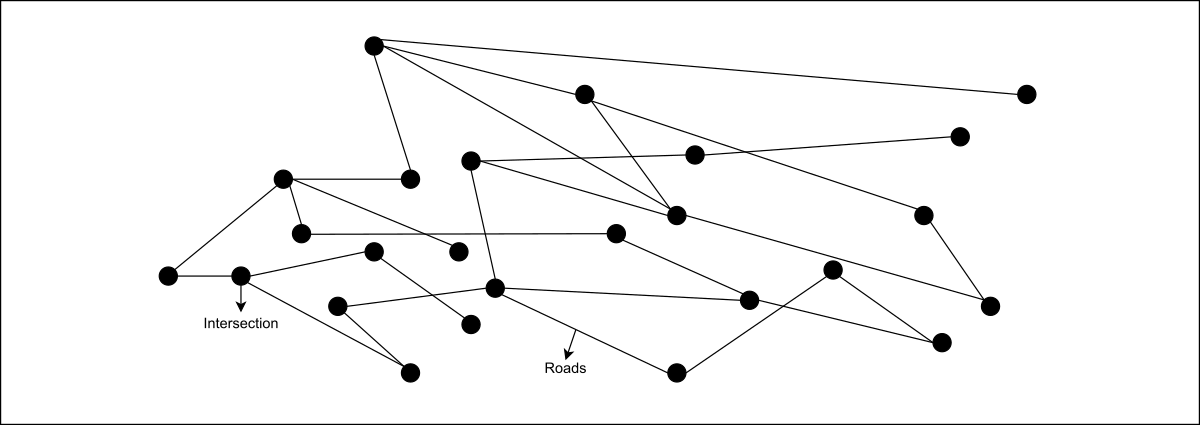
\includegraphics[width=0.5\textwidth]{Images/chapter_30/section_6683135341494272/5817979795406848.png}
 \caption{Graph representation}
\end{figure}

To identify the shortest path between source and destination, we can utilize routing algorithms such as Dijkstra's algorithm. However, Dijkstra, or any other algorithm that operates on top of an unprocessed graph, is quite slow for such a system. Therefore, this method is impractical at the scale at which these ride-hailing platforms operate.
\\
To resolve these issues, we can split the whole graph into partitions. We preprocess the optimum path inside partitions using \textbf{contraction hierarchies}(Contraction hierarchies is a speed-up method optimized to exploit the properties of graphs representing road networks. The speed-up is achieved by creating shortcuts in a preprocessing phase, which are then used during a shortest-path query to skip over unimportant vertices. Source: Wikipedia) and deal with just the partition boundaries. This strategy can considerably reduce the time complexity since it partitions the graph into layers of tiny cells that are largely independent of one another. The preprocessing stage is executed in parallel in the partitions when necessary to increase speed. In the illustration below, all the partitions process the best route in parallel. For example, if each partition takes one second to find the path, we can have the complete path in one second since all partitions work in parallel.

\begin{figure}[htbp]
 \centering
 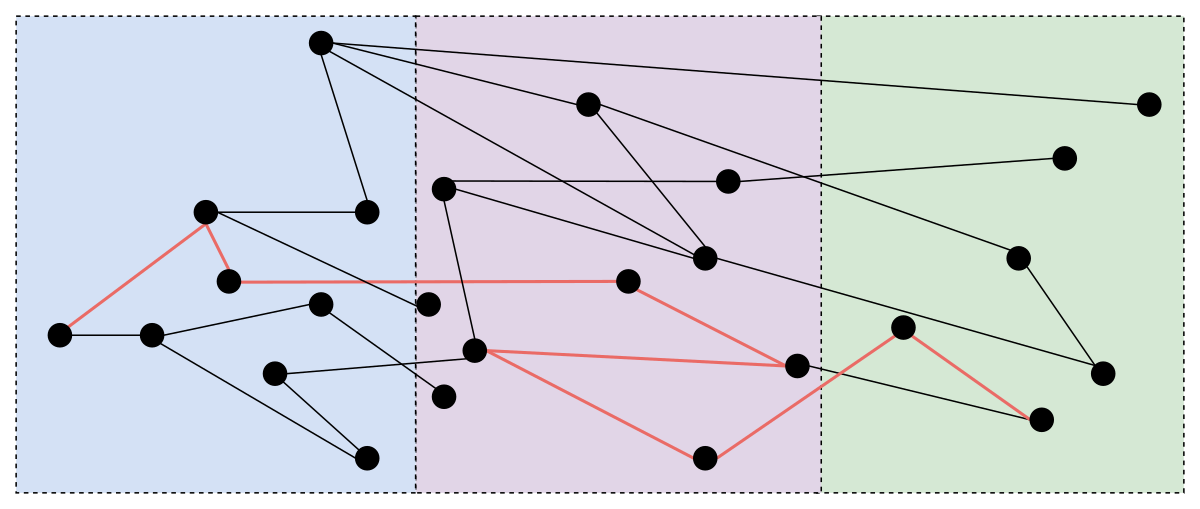
\includegraphics[width=0.5\textwidth]{Images/chapter_30/section_6683135341494272/4558668431622144.png}
 \caption{Partitioning the graph}
\end{figure}

Once we determine the best route, we calculate the expected time to travel the road segment while accounting for traffic. The traffic data will be the edge weights between the nodes.
\\
\paragraph{DeepETA}\label{OUucURq-m_YBVYF0pGXva}
\\
We use a machine learning component named \textbf{DeepETA} to deliver an immediate improvement to metrics in production. It establishes a model foundation that can be reused for multiple consumer use cases.
\\
We also use a routing engine that uses real-time traffic information and map data to predict an ETA to traverse the best path between the source and the destination. We use a post-processing ML model that considers spatial and temporal parameters, such as the source, destination, time of the request, and knowledge about real-time traffic, to forecast the ETA residual.

\begin{figure}[htbp]
 \centering
 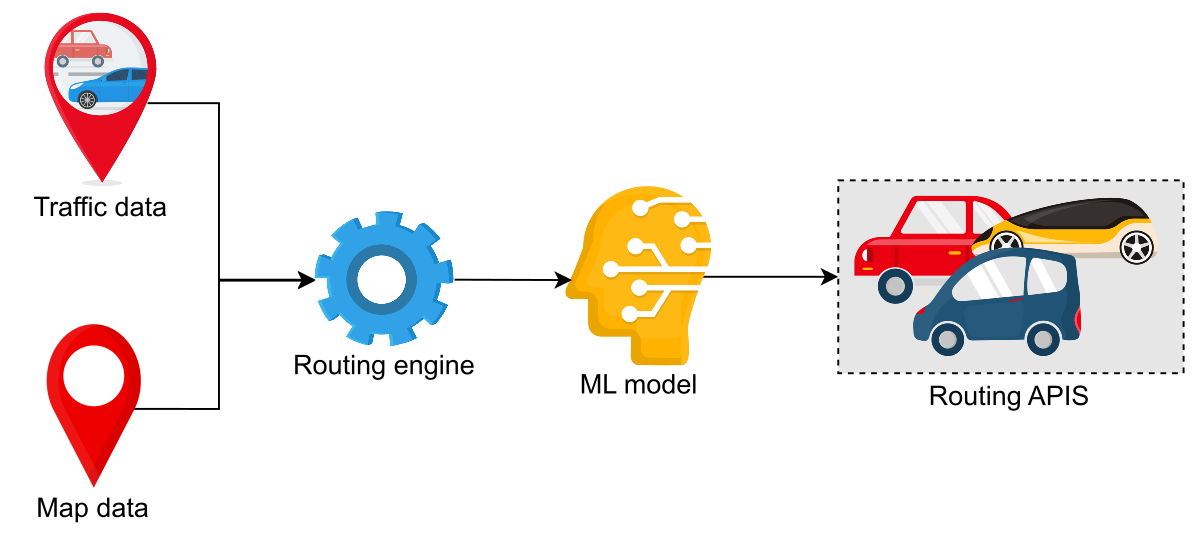
\includegraphics[width=0.5\textwidth]{Images/chapter_30/section_6683135341494272/4528288752205824.png}
 \caption{DeepETA}
\end{figure}

\subsubsection{Database}\label{kRiu6n_YV_i7I7Uimai_q}
\\
Let's select the database according to our requirements:

\begin{itemize}
\item
\protect\phantomsection\label{44vPZCTPcoNaanAhQUam0}
The database must be able to scale horizontally. There are new customers and drivers on a regular basis, so we should be able to add more storage without any problems.
\item
\protect\phantomsection\label{tMmYZFcc73V1otgHcvLh5}
The database should handle a large number of reads and writes because the location of drivers is updated every four seconds.
\item
\protect\phantomsection\label{mTLqdCfdiDds0KaebJ2gd}
Our system should never be down.
\end{itemize}
\\
We've already discussed the various database types and their specifications in the \href{https://www.educative.io/courses/grokking-the-system-design-interview/introduction-to-databases}{Database} chapter. So , according to our understanding and requirements (high availability, high scalability, and fault tolerance), we can use Cassandra(Cassandra is a columnar database, which is a type of NoSQL database designed to handle large amounts of data across many commodity servers, providing high availability with no single point of failure. Source
: Wikipedia) to store the driver's last known location and the trip information after the trip has been completed, and there will be no updates to it. We use Cassandra because the data we store is enormous and it increases continuously.
\\
We can use a MySQL database to store trip information while it's in progress. We use MySQL for in-progress trips for frequent updates since the trip information is relational, and it needs to be consistent across tables.
\begin{quote}
\textbf{Note:} Recently, Uber migrated their data storage to Google Cloud Spanner. It provides global transactions, strongly consistent reads, and automatic multisite replication and failover features.
\end{quote}
\\
We're using both MySQL and Cassandra databases in Uber's design. Why can't we use \textbf{only} MySQL or \textbf{only} a Cassandra database? In other words, what is the need for using both databases?

\textbf{Question:}

Why can't we use only MySQL or only a Cassandra database? 

\textbf{Reference Answer:}

The data we store for each trip is highly relational, it's spread over multiple tables, and it must be identical among all tables. My SQL helps to store this relational data and keep it consistent across tables.
\\
As the data becomes massive with the passage of time, it reduces our system's performance. Also , it won't be easy to scale the MySQL database. Hence we use Cassandra to store the driver's last known location and the trip information after the trip has been completed.

\paragraph{Storage schema}\label{9OIhjDmVrK-ed35mH6CLc}
\\
On a basic level, in the Uber application, we need the following tables:

\begin{itemize}
\item
\protect\phantomsection\label{tWZ6rdKKIbDee7MQY2Tb9}
\textbf{Riders:} We store the rider's related information, such as ID, name, email, photo, phone number, and so on.
\item
\protect\phantomsection\label{7KlWr0MMtkhk-39rTlVp6}
\textbf{Drivers:} We store the driver's related information, such as ID, name, email, photo, phone number, vehicle name, vehicle type, and so on.
\item
\protect\phantomsection\label{sogsvR-moLN8TToM-ty8X}
\textbf{Driver\_location:} We store the driver's last known location.
\item
\protect\phantomsection\label{AmA0SFoRxTIOcXLun7ny6}
\textbf{Trips:} We store the trip's related information, such as trip ID, rider ID, driver ID, status, ETA, location of the vehicle, and so on.
\end{itemize}
\\
The following illustration visualizes the data model:

\begin{figure}[htbp]
 \centering
 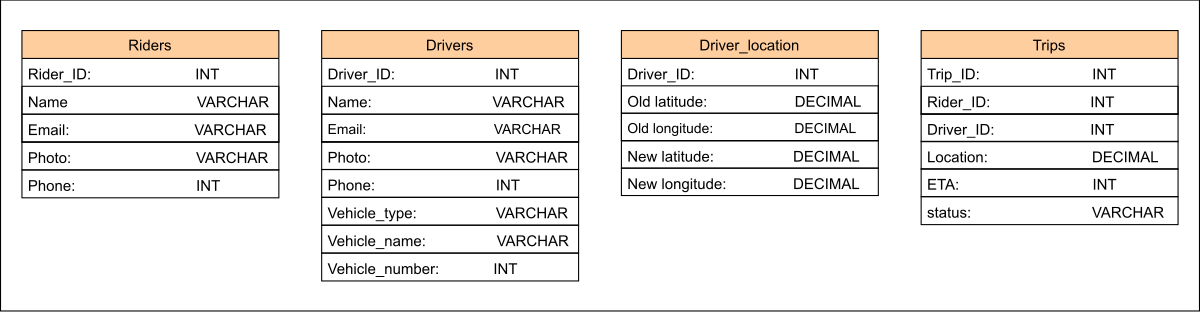
\includegraphics[width=0.5\textwidth]{Images/chapter_30/section_6683135341494272/4907573388247040.png}
 \caption{The storage schema}
\end{figure}

\subsubsection{Fault tolerance}\label{i3s3rgbIzvEI1Qv82a8hL}
\\
For availability, we need to have replicas of our database. We use the primary-secondary replication model. We have one primary database and a few secondary databases. We synchronously replicate data from primary to secondary databases. Whenever our primary database is down, we can use a secondary database as the primary one.

\begin{quote}
\textbf{Quiz:}
\textbf{Question 1:} How will we handle a driver\textquotesingle s slow and disconnecting network?
\textbf{Answer:} We can use the driver's phone as local storage and save the state of a trip every few seconds there. All requests and the last recorded state are stored on a local disk, which ensures that they're preserved even if the application is restarted. Suppose the driver exits the application while there are a few requests waiting to be synchronized with the server. The requests and last known state are loaded from the local disk upon relaunch. When the driver relaunches the application, they remain in the same situation as before. The requests are queued in order to keep the server up to date.
\end{quote}

\subsubsection{Load balancers}\label{B9XSXfnn4-WjpOEMrVI49}
\\
We use load balancers between clients (drivers and riders) and the application servers to uniformly distribute the load among the servers. The requests are routed to the specified server that provides the requested service.

\subsubsection{Cache}\label{f39daXdyf4lT6QN_uBE5z}
\\
A million drivers need to send the updated location every four seconds. A million requests to the QuadTree service affects how well it works. For this, we first store the updated location in the hash table stored in Redis. Eventually , these values are copied into the persistent storage every 10--15 seconds.
\\
We've discussed the detailed design of Uber and how different components work together to fulfill the requirements. In the next lesson, we'll learn how the payment service works to move the money from riders to drivers and detect frauds.

% End of section content